% !TEX TS-program = pdflatex
% !TEX encoding = UTF-8 Unicode

\documentclass[10pt, a4paper]{article}

% Essential packages
\usepackage[utf8]{inputenc}
\usepackage[T1]{fontenc}
\usepackage{helvet}
\usepackage{amssymb}
\usepackage{graphicx}
\renewcommand{\familydefault}{\sfdefault}

% Page geometry for landscape layout
\usepackage{geometry}
\geometry{a4paper, landscape, margin=1cm, top=1cm, bottom=1.5cm}

% Colors for box styling
\usepackage{xcolor}
\definecolor{boxheaderbg}{HTML}{000000}
\definecolor{boxheaderfg}{HTML}{FFFFFF}
\definecolor{boxcontentbg}{HTML}{F0F0F0}
\definecolor{boxborder}{HTML}{000000}

% tcolorbox for fixed-size boxes
\usepackage[many]{tcolorbox}

% hyperref for form fields
\usepackage{hyperref}

% Headers and footers
\usepackage{fancyhdr}
\pagestyle{fancy}
\fancyhf{}
\fancyfoot[R]{\footnotesize "Fail Forward character sheet" by Visa Lampi is licensed under CC BY-NC 4.0.}
\renewcommand{\headrulewidth}{0pt}
\renewcommand{\footrulewidth}{0pt}

% Tabularx for table formatting
\usepackage{tabularx}

\begin{document}

% Start of the form
\begin{Form}

% Two-column layout with minipages
\begin{minipage}[t]{0.48\textwidth}
    \vspace{0pt}
    % Character box with adjusted image positioning and scaling
    \begin{tcolorbox}[
        width=12.5cm,
        height=4.5cm,
        title=CHARACTER,
        colback=boxcontentbg,
        colframe=boxborder,
        coltitle=boxheaderfg,
        colbacktitle=boxheaderbg,
        fonttitle=\bfseries\sffamily\small,
        clip upper,
        before skip=0pt
    ]
        \begin{minipage}[t][4cm]{0.22\linewidth}
            \centering
            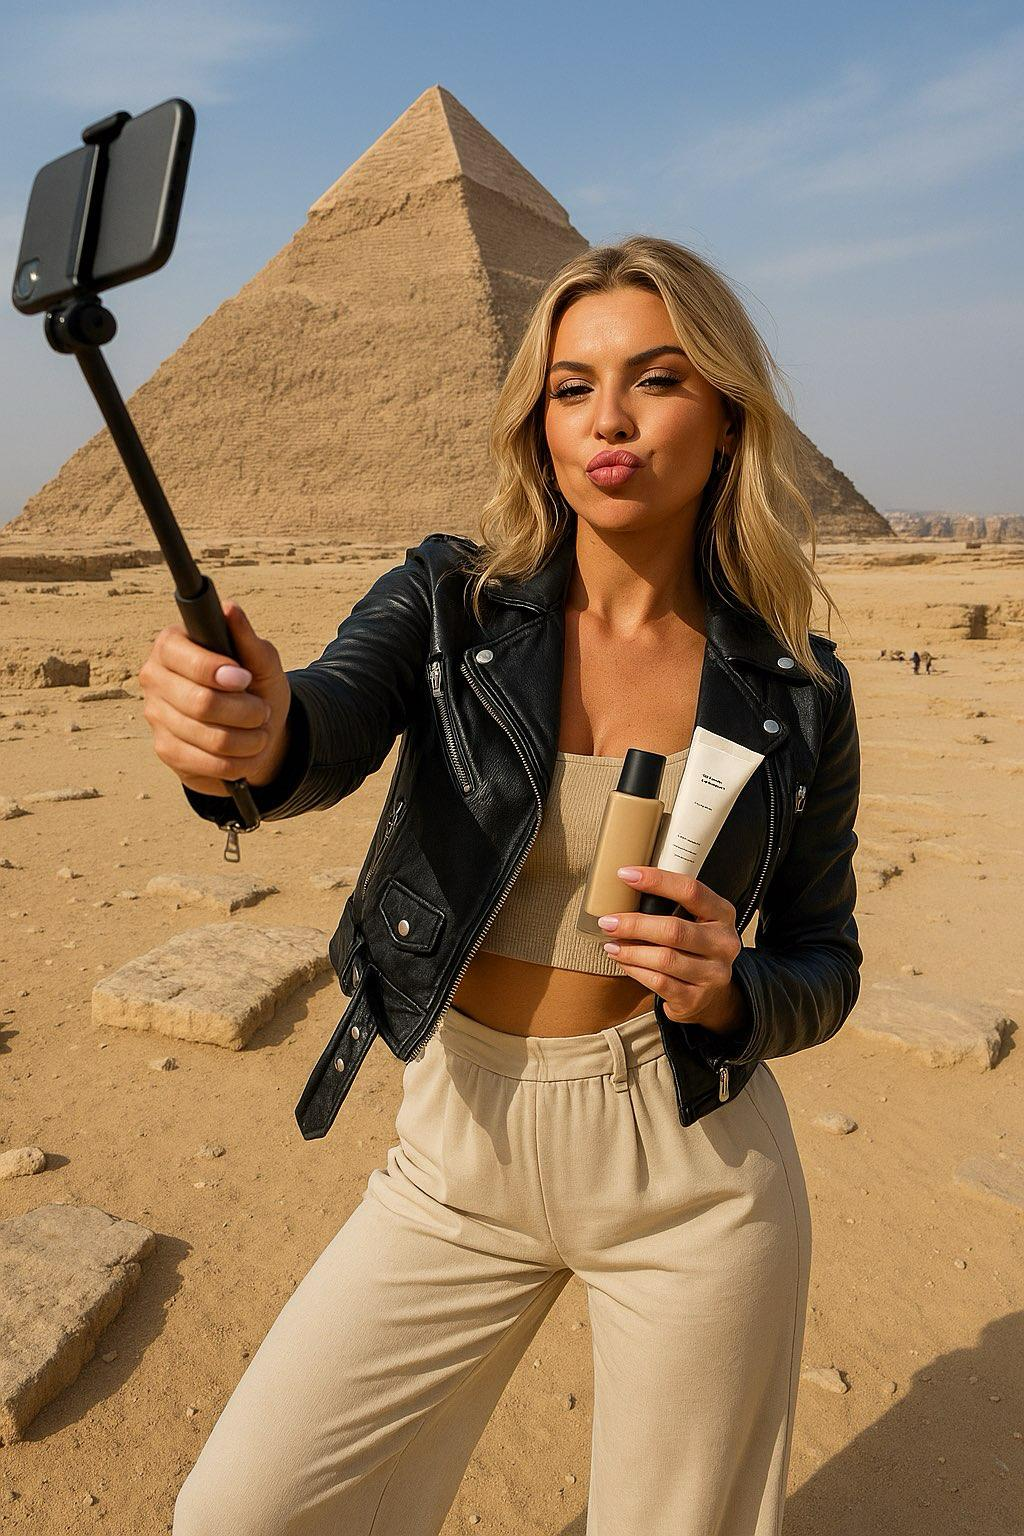
\includegraphics[width=0.9\linewidth, height=3.8cm, keepaspectratio=true]{Saphire.jpg}
            \vspace{0pt}
        \end{minipage}%
        \hspace{0.2cm}%
        \begin{minipage}[t][4cm]{0.74\linewidth}
            \centering
            \TextField[name=character_name, width=8cm, height=2cm, multiline=true, default={Sapphire Skye Monroe @sapphireontherise}, charsize=20pt, backgroundcolor=boxcontentbg, borderwidth=0, bordercolor=boxcontentbg]{}
        \end{minipage}
    \end{tcolorbox}

    \vspace{3mm}

    % Background box with updated bio
    \begin{tcolorbox}[
        width=12.5cm,
        height=6.5cm,
        title=BACKGROUND,
        colback=boxcontentbg,
        colframe=boxborder,
        coltitle=boxheaderfg,
        colbacktitle=boxheaderbg,
        fonttitle=\bfseries\sffamily\small,
        clip upper,
        before skip=0pt
    ]
        \TextField[name=background, width=11.5cm, height=5.5cm, multiline=true, default={To her 3.2M TikTok followers, @sapphireontherise is a hilariously clueless "Spiritual CEO." In reality, it's a carefully crafted act. Sapphire's parents were respected academics ruined for their controversial theories on Atlantis. Now, she uses her influencer income to fund a secret investigation into their work, playing the fool to get access to sites and information that would be denied to anyone taking the subject seriously. Her true goal is to find the proof that will vindicate her family's name. \newline \newline \textbf{Personal Quest:} To find the "Atlantean Star-Chart" her parents were searching for when they were discredited, believing it's the ultimate proof of their theories. \newline \textbf{Key Contact:} Dr. Miles Corbin, her parents' most loyal (and now disgraced) colleague, who guides her research from the shadows.}, backgroundcolor=boxcontentbg, borderwidth=0, bordercolor=boxcontentbg]{}
    \end{tcolorbox}

    \vspace{3mm}

    % Abilities box with updated abilities
    \begin{tcolorbox}[
        width=12.5cm,
        height=4cm,
        title=ABILITIES (choose 3),
        colback=boxcontentbg,
        colframe=boxborder,
        coltitle=boxheaderfg,
        colbacktitle=boxheaderbg,
        fonttitle=\bfseries\sffamily\small,
        clip upper,
        before skip=0pt
    ]
        \TextField[name=abilities, width=11.5cm, height=3cm, multiline=true, default={\newlinechar Social Media Savvy \qquad \hspace{10mm} Influencer Charisma \newline \qquad \newline Historical Misinterpretation \qquad Wellness Product Promotion Yoga & Meditation}, backgroundcolor=boxcontentbg, borderwidth=0, bordercolor=boxcontentbg]{}
    \end{tcolorbox}
\end{minipage}
\hfill
\begin{minipage}[t]{0.48\textwidth}
    \vspace{0pt}
    % Sanity box (unchanged)
    \begin{tcolorbox}[
        width=12.5cm,
        height=2.5cm,
        title=SANITY,
        colback=boxcontentbg,
        colframe=boxborder,
        coltitle=boxheaderfg,
        colbacktitle=boxheaderbg,
        fonttitle=\bfseries\sffamily\small,
        clip upper,
        before skip=0pt
    ]
        \begin{minipage}[t]{\linewidth}
            \large \hspace*{2mm}
            $\bigcirc$ \hspace{1em}
            $\bigcirc$ \hspace{1em}
            $\bigcirc$ \hspace{1em}
            $\bigcirc$ \hspace{1em}
            $\bigcirc$ \hspace{1em}
            $\bigcirc$ \\
            \textit{\footnotesize \hspace*{2mm} (6 = Sanity breaks)} \\
            \vspace{2mm}
            \textit{\footnotesize \hspace*{2mm} Check one circle each time sanity decreases.}
        \end{minipage}
    \end{tcolorbox}

    \vspace{3mm}

    % Personality box with updated personality traits
    \begin{tcolorbox}[
        width=12.5cm,
        height=3.5cm,
        title=PERSONALITY (choose 2),
        colback=boxcontentbg,
        colframe=boxborder,
        coltitle=boxheaderfg,
        colbacktitle=boxheaderbg,
        fonttitle=\bfseries\sffamily\small,
        clip upper,
        before skip=0pt
    ]
        \TextField[name=personality, width=11.5cm, height=2.5cm, multiline=true, default={Charismatic  Eccentric}, backgroundcolor=boxcontentbg, borderwidth=0, bordercolor=boxcontentbg]{}
    \end{tcolorbox}

    \vspace{3mm}

    % Handicaps box with updated handicaps
    \begin{tcolorbox}[
        width=12.5cm,
        height=3.5cm,
        title=SANITY UNDER STRESS (choose 2),
        colback=boxcontentbg,
        colframe=boxborder,
        coltitle=boxheaderfg,
        colbacktitle=boxheaderbg,
        fonttitle=\bfseries\sffamily\small,
        clip upper,
        before skip=0pt
    ]
        \TextField[name=handicaps, width=11.5cm, height=2.5cm, multiline=true, default={Persona Inversion \quad Device Paranoia \quad Reckless Vindication \newline Auditory Scorn}, backgroundcolor=boxcontentbg, borderwidth=0, bordercolor=boxcontentbg]{}
    \end{tcolorbox}

    \vspace{3mm}

    % Equipment box with updated equipment
    \begin{tcolorbox}[
        width=12.5cm,
        height=5cm,
        title=EQUIPMENT (choose 4),
        colback=boxcontentbg,
        colframe=boxborder,
        coltitle=boxheaderfg,
        colbacktitle=boxheaderbg,
        fonttitle=\bfseries\sffamily\small,
        clip upper,
        before skip=0pt
    ]
        \TextField[name=equipment, width=11.5cm, height=4cm, multiline=true, default={Smartphone  Crystal Water Bottle  Selfie Stick  Designer Sunglasses  Mushrooms  Smoke Grenades  Derringer \quad Blessed Scarab \quad Ancient Coin \quad Strange Idol \quad Polaroid Camera}, backgroundcolor=boxcontentbg, borderwidth=0, bordercolor=boxcontentbg]{}
    \end{tcolorbox}
\end{minipage}

% End of the form
\end{Form}

\end{document}